\documentclass[12pt]{article}%
\usepackage{amsfonts}
\usepackage{fancyhdr}
\usepackage{comment}
\usepackage{graphicx}
\usepackage{float}
\usepackage{wrapfig}

\usepackage[a4paper, top=2.5cm, bottom=2.5cm, left=2.2cm, right=2.2cm]%
{geometry}
\usepackage{times}
\usepackage{amsmath}
\usepackage{enumitem}
\usepackage{amsfonts}
\usepackage{titlesec}
\usepackage{pst-node}

\setcounter{secnumdepth}{0}

\usepackage{tikz-cd} 
\usepackage{changepage}
\usepackage{amssymb}
\usepackage{graphicx}%
\setcounter{MaxMatrixCols}{30}
\newtheorem{theorem}{Theorem}
\newtheorem{acknowledgement}[theorem]{Acknowledgement}
\newtheorem{algorithm}[theorem]{Algorithm}
\newtheorem{axiom}{Axiom}
\newtheorem{case}[theorem]{Case}
\newtheorem{claim}[theorem]{Claim}
\newtheorem{conclusion}[theorem]{Conclusion}
\newtheorem{condition}[theorem]{Condition}
\newtheorem{conjecture}[theorem]{Conjecture}
\newtheorem{corollary}[theorem]{Corollary}
\newtheorem{criterion}[theorem]{Criterion}
\newtheorem{definition}[theorem]{Definition}
\newtheorem{example}[theorem]{Example}
\newtheorem{exercise}[theorem]{Exercise}
\newtheorem{lemma}[theorem]{Lemma}
\newtheorem{notation}[theorem]{Notation}
\newtheorem{problem}[theorem]{Problem}
\newtheorem{proposition}[theorem]{Proposition}
\newtheorem{remark}[theorem]{Remark}
\newtheorem{solution}[theorem]{Solution}
\newtheorem{summary}[theorem]{Summary}
\newenvironment{proof}[1][Proof]{\textbf{#1.} }{\ \rule{0.5em}{0.5em}}

\newcommand{\Q}{\mathbb{Q}}
\newcommand{\R}{\mathbb{R}}
\newcommand{\C}{\mathbb{C}}
\newcommand{\Z}{\mathbb{Z}}
\newcommand{\N}{\mathbb{N}}
\newcommand{\nsg}{\underline{$\lhd$} }
\newcommand{\qed}{\blacksquare}

\newcommand{\Sen}{\mathcal{S}}
\newcommand{\Rec}{\mathcal{R}}

\title{CS880: Final Project Report}
\author{Ansh Aggarwal $\quad$ Rohan Chakravarthi $\quad$ Yijun Zhu}
\date{}
\begin{document}
\maketitle
\vspace{10.0cm}
\section{Abstract}
Error detection and correction (EDAC) schemes are techniques used to detect, mitigate, and correct errors over inconsistent and unreliable communication channels. Often, the number of errors that can be introduced through these channels are considered to be unbounded, however, with the advent of modern communication systems, this outlook may be considered pessimistic. As such, it is worth looking into EDAC schemes that surpass information-theoretic limits for errors that are computationally bounded. The work of Jad Silbak and Daniel Wichs across two papers: \textit{Detecting and Correcting Computationally Bounded Errors: A Simple Construction Under Minimal Assumptions} [2024] and \textit{Binary Codes for Error Detection and Correction
in a Computationally Bounded World} [2025] explores constructions for EDAC schemes under the aforementioned setting. We highlight and explore the findings and constructions from Silbak and Wichs' work in this survey. \newpage 

\tableofcontents

\section{Introduction}
The two objects that fall under EDAC are error detection codes (EDC) and error correction codes (ECC) with two different objectives. Consider the following setup: let $\Sen$ be the sender and let $\Rec$ be the receiver, and let $m_s$ be the message that $\Sen$ would like to send to $\Rec$ and let $m'$ be the message that $\Rec$ receives. \begin{enumerate}
    \item The goal of error detection is to allow $\Rec$ to verify whether $m = m'$
    \item The goal of error correction is to allow $\Rec$ to recover $m$ from $m'$ even if $m \not = m'$
\end{enumerate} 

\subsection{Notation and EDAC Basics}

\subsubsection{Alphabet}
The alphabet for a code refers to the set of symbols that may be used to construct the code. This set is represented with $[q]$ where $q$ is number of symbols in that set. Note that if the alphabet is simply $\{0, 1\}$, then the code is called a binary code.

\subsubsection{Hamming Distance}
\noindent The central metric for EDAC schemes is Hamming distance: for $x, y \in [q]^n$, we have \begin{align}
    \Delta(x, y) = |\{i \mid x_i \neq y_i\}|
\end{align} Another notion is the relative Hamming distance which is simply $\delta(x, y) = \Delta(x, y) / n$. For example, for the words \textit{cat}, \textit{dog}, and \textit{god} in the standard English alphabet, we have $\Delta$(cat, dog) $ = 3$, $\Delta$(cat, god) $ = 3$, and $\Delta$(god, dog) $ = 2$.  

\subsubsection{Code Syntax}

Let $k, n, q$ be parameters and let \textsf{Encode}$:\{0, 1\}^k \to [q]^n$ be a function. \textsf{Encode} is an encoding function that: \begin{enumerate}
    \item Decode $d$ errors: If $\exists$ $\textsf{Decode}:[q]^n \to \{0, 1\}^k$ such that for $m \in \{0, 1\}^k$ and $v \in [q]^n$, if $\Delta(\textsf{Encode}(m), v) \leq d$, then \textsf{Decode}$(v) = m$
    \item Detect $d$ errors: If $\exists$ $\textsf{Decode}: [q]^n \to \{\bot\} \cup\{0, 1\}^k$ such that for $m \in \{0, 1\}^k$ and $v \in [q]^n$, and $\textsf{Encode}(m) \neq v$ but $\Delta(\textsf{Encode}(m), v) \leq d$, then \textsf{Decode}$(v) = \bot$
\end{enumerate} Additionally, some codes include a notion of $L$-list-decodes where $\textsf{Decode}$ is allowed to output up to $L$ values and for $m \in \{0, 1\}^k$ and $v \in [q]^n$, if $\Delta(\textsf{Encode}(m), v) \leq d$, then $m \in \textsf{Decode}(v)$. In essence, this means the decode function outputs a list of potential decodes instead of outputting a single decode for a given codeword. 

\subsubsection{Rate and Error Tolerance}

 EDAC schemes are assessed primarily on the basis of two parameters: \begin{enumerate}
    \item The rate of the code is $R$ where $R = \frac{k}{n \log q}$ where $k$ is number of message bits and $n$ is number of redundancy / code bits and $q$ is the size of the alphabet. Note that for binary codes, this is simply $R = k/n$ 
    \item The relative error tolerance, $\rho$, of a code is the ratio of the number of errors a code can handle, $d$, and the number of bits in the code word, $n$ thus, $\rho = \frac{d}{n}$; it should be noted that $\rho \leq 1/2$ for error correction and $\rho \leq 1$ for error detection 
\end{enumerate}

\subsubsection{Communication Channels}

Essentially, a communication channel is the medium that is used to transmit the message from $\Sen$ to $\Rec$. In the real world, this could range from carrier pigeons to using semaphores but in context of these papers (and generally EDAC schemes), we're usually referring to digital transmission methods. When EDAC schemes were studied during its pioneering days in the 1940s, the standard transmission methods were extremely lossy and inconsistent and as such, the amount of errors that communication channel could introduce during transmission was considered to be unbounded. With the introduction of more reliable communication channels, a natural modification to this assumption is to make errors bounded and as the work that we explore finds, this allows EDAC schemes to approach theoretically optimal limits, that is $\rho \approx1$ and $\rho \approx 1/2$ for detection and correction respectively. In work related to error correcting codes, the notion of an adversarial channel is used which, as the name might suggest, picks the worst-case message for any given scheme/construction in order to make it decode a code word incorrectly. This notion is used throughout the papers and is assumed in this survey as well. 

\subsubsection{Singleton Bound}
For linear codes, the Singleton bound is an upper bound for the number of codes for a given code with alphabet $[q]$ that is tighter than the trivial $q^n$ bound. This implies that for any rate $R \geq 0$, we have that $\rho \leq 1 - R$ for detection and $\rho \leq \frac{1}{2}(1 - R)$. 
 
\subsubsection{Blokh-Zyablov Bound}
The Blokh-Zyablov bound gives a bound for the best-known information theoretic rate $R$ and error tolerance $p$ for efficiently list-decodable binary codes. 


\subsection{Primitives}
This is a generalized overview of assumptions and primitives that are used across both papers that include fairly standard assumptions like one way functions but also some far more exotic ones like \textit{crypto dark matter}. These definitions are taken from the original papers for consistency. 

\subsubsection{One Way Functions}

A probabilistic polynomial-time (PPT) algorithm $F:\{0, 1\}^* \to \{0, 1\}^*$ is a one-way function if for every PPT adversary and every sufficiently large $k \in \N$, we have: $$\textbf{Pr}_{x \xleftarrow{} \{0, 1\}^k}[A(1^k, F(x)) \in F^{-1}(F(x))] \leq \textsf{negl}(k)$$ In simple terms, given $F(x)$, it is hard for a polynomial time adversary to find $x$. 

\subsubsection{Universal One Way Hash Functions}

For a security parameter $k \in N$. A family of functions $\mathcal{H} = \{h_s: \{0, 1\}^{n(k) } \to \{0, 1\}^{l(k)}\})_{s \in \{0, 1\}^{l(k)}}$ is a family of universal one way hash functions if it satisfies: \begin{enumerate}
    \item Efficiency: Given $s \in \{0, 1\}^{l(k)}$ and $x \in \{0, 1\}^{n(k)}$, $h_s(x)$ can be evaluated in time poly$(n(k), l(k))$
    \item Shrinking: $l(k) < n(k)$
    \item Target Collision Resistance: For every PPT adversary and sufficiently large $k \in \N$, if we consider the following randomized experiment: \begin{enumerate}
        \item ($x$, state) $\xleftarrow{} A(1^k) \in \{0, 1\}^{n(k)} \times \{0, 1\}^*$
        \item Sampling $s \xleftarrow{} \{0, 1\}^{l(k)}$
        \item $x' \xleftarrow{} A($state, $s)$
    \end{enumerate} Then \textbf{Pr}$[x \neq x' \text{ and } h_s(x) = h_s(x')] \leq \textsf{negl}(k)$
\end{enumerate}

\subsubsection{Collision Resistant Hash Functions}

For a security parameter $k \in N$. A family of functions $\mathcal{H} = \{h_s: \{0, 1\}^{n(k) } \to \{0, 1\}^{l(k)}\})_{s \in \{0, 1\}^{l(k)}}$ is a family of universal one way hash functions if it satisfies: \begin{enumerate}
    \item Efficiency: Given $s \in \{0, 1\}^{l(k)}$ and $x \in \{0, 1\}^{n(k)}$, $h_s(x)$ can be evaluated in time poly$(n(k), l(k))$
    \item Shrinking: $l(k) < n(k)$
    \item Collision Resistance: For every PPT adversary and sufficiently large $k \in \N$, $$\textbf{Pr}_{s \xleftarrow{} \{0, 1\}^k; x, x' \xleftarrow{} A(s)} [x \neq x' \text{ and } h_s(x) = h_s(x')] \leq \textsf{negl}(k)$$
\end{enumerate} The main difference between UOWHFs and CRHFs is the third requirement where the difference is that UOWHFs fix $x$ and an output and demand the adversary come up with another $x'$ such that the outputs match while collision resistance demands that the adversary come up with two distinct message that have the same output.


\subsubsection{Correlation Intractability Hashing}

Let $k \in \N$ be a security parameter and $t \in $ poly be a poly-time computable function. The hash family $\mathcal{H} = \{h_s:\{0, 1\}^{n(k)} \to \{0, 1\}^{m(k)}\}_{s \in \{0, 1\}^{l(k)}}$ is correlation intractable for $t$-size circuits ($t$-CI) if for every size$(t)$ circuit family $f = \{f_k: \{0, 1\}^{n(k)} \to (\{0, 1\}^{m(k)})^{L(k)}\}_{k \in \N}$ whose output is interpreted as a set, and every (non-uniform) PPT adversary $A$: $$\textbf{Pr}_{s \xleftarrow{} \{0, 1\}^{l(k)}; x \xleftarrow{} A(s)} [h_s(x) \in f_k(x)] \leq \textsf{negl}(k)$$ In simpler terms, a hash family $\mathcal{H}$ is $t$-CI for a spare relationship $R(x, y)$ if given a random seed $s \xleftarrow{} \{ 0,1\}$, it is computationally hard to find an $x$, such that $(x, h_s(x)) \in R$. A spare relationship, loosely, means that elements contained in it have very few or no special algebraic relationships or patterns that link them. This is not formal, but I believe this is a notion similar to the idea of perfect secrecy in that it says that given some hash output, the probability that it was computed from $m$ is the same as the probability it was computed from some other $m'$. 

\subsubsection{Random Oracle Model}

The Random Oracle Model (ROM) is an idealized cryptographic model in which a hash function $H : \{0,1\}^* \to \{0,1\}^m$ is treated as a truly random function. Formally, there exists a public oracle $\mathcal{O}_H$ such that:

\[
\mathcal{O}_H(x) = 
\begin{cases}
y, & \text{if } x \text{ has been queried before and } \mathcal{O}_H(x) = y \text{ was recorded} \\
y \xleftarrow{\$} \{0,1\}^m, & \text{if } x \text{ is a new query}
\end{cases}
\]

The oracle maintains a table of previous queries and outputs. For every new query $x$, the output $y$ is sampled uniformly at random from $\{0,1\}^m$ and stored. The oracle is deterministic from the adversary's perspective: repeated queries always return the same output.

In this model, all parties—including the adversary—have oracle access to $H$ through $\mathcal{O}_H$. The ROM enables proofs of cryptographic security under the assumption that $H$ behaves like an ideal random function.

\subsubsection{Target 2-Input Correlation Intractability Hashing}

\textbf{Definition}\\

Let $k \in \N$ be a security parameter and $t \in $ poly be a poly-time computable function. The hash family $\mathcal{H} = \{h_s:\{0, 1\}^{n(k)} \to \{0, 1\}^{m(k)}\}_{s \in \{0, 1\}^{l(k)}}$ is target $2$-input correlation intractable for $t$-size ($t$-T2CI) is for every $L \in $ poly, size$(t)$ circuit $f = \{f_k:\{0, 1\}^{n(k)} \times \{0, 1\}^{n(k)} \times \{0, 1\}^{m(k)} \to (\{0, 1\}^{m(k)})^{L(k)}\}_{k \in \N}$ and every PPT adversary $A$, if we consider the experiment: \begin{enumerate}
    \item ($x$, state) $\xleftarrow{} A(1^k) \in \{0, 1\}^{n(k)} \times \{0, 1\}^*$
    \item Sampling $s \xleftarrow{} \{0, 1\}^{l(k)}$
    \item $x' \xleftarrow{} A($state, $s)$
\end{enumerate} Then \textbf{Pr}$[h_s(x') \in f_k(x' , x, h_s(x)) \text{ and } x' \neq x] \leq \textsf{negl}(k)$. The main goal of $t$-T2CI from $t$-CI is that we'd like intractability to hold for two pairs of hash computations simultaneously. The authors construct T2CI from CI and UOWHFs which they build using the LWE assumption.

\paragraph{Construction.}

We construct a $t$-T2CI hash family $\mathcal{H}$ from two well-established cryptographic primitives:

\begin{itemize}
    \item A \textbf{correlation intractable (CI)} hash family:
    \[
    \mathcal{H}_{\mathrm{CI}} = \{h^{\mathrm{CI}}_{s_1} : \{0,1\}^{n(k)} \to \{0,1\}^{m_1(k)}\}_{s_1 \in \{0,1\}^{\ell_1(k)}}
    \]
    This is a family of hash functions parameterized by a seed $s_1$, where each function takes an input of length $n(k)$ and maps it to an output of length $m_1(k)$. Correlation intractability ensures that it is hard for an adversary to find an input $x$ that satisfies some circuit-defined relation $R(x, h^{\mathrm{CI}}_{s_1}(x)) = 1$.

    \item A \textbf{universal one-way hash family (UOWHF)}:
    \[
    \mathcal{H}_{\mathrm{UOWHF}} = \{h^{\mathrm{UOWHF}}_{s_2} : \{0,1\}^{n(k)} \to \{0,1\}^{m_2(k)}\}_{s_2 \in \{0,1\}^{\ell_2(k)}}
    \]
    This is a family of hash functions where, even if an adversary chooses a fixed input $x$, it is computationally infeasible to find a different $x' \ne x$ such that $h^{\mathrm{UOWHF}}_{s_2}(x') = h^{\mathrm{UOWHF}}_{s_2}(x)$. The UOWHF component prevents output collisions on related or distinct inputs.
\end{itemize}

We define the composed hash function $h_s$ in the T2CI family $\mathcal{H}$ as the concatenation of the two components:
\[
\mathcal{H} = \left\{ h_s(x) = h^{\mathrm{CI}}_{s_1}(x) \, \| \, h^{\mathrm{UOWHF}}_{s_2}(x) \right\}_{s = (s_1, s_2)}
\]

\begin{itemize}
    \item The overall seed $s$ is the tuple $(s_1, s_2)$, combining the seeds of the two subcomponents.
    
    \item The function $h_s(x)$ outputs a string of length $m_1(k) + m_2(k)$ by concatenating the outputs of the CI and UOWHF hash functions applied to the same input $x$. This ensures the combined output carries both types of cryptographic hardness properties.
\end{itemize}

\paragraph{Step-by-step justification:}

\begin{enumerate}
    \item \textbf{Correlation intractability from $h^{\mathrm{CI}}$:} The purpose of using the CI hash function is to prevent an adversary from producing inputs $x$ that satisfy a predetermined circuit-based relation involving the hash output. This is crucial for the \textit{“target”} aspect of T2CI: the adversary is given $(x, h_s(x))$ and must not be able to find $x' \ne x$ such that $h_s(x')$ satisfies some computable relation involving $x$, $x'$, and $h_s(x)$. Without this component, correlation-based attacks would be feasible.

    \item \textbf{Second preimage resistance from $h^{\mathrm{UOWHF}}$:} The UOWHF component ensures that once $x$ is fixed, an adversary cannot find $x' \ne x$ such that $h^{\mathrm{UOWHF}}_{s_2}(x') = h^{\mathrm{UOWHF}}_{s_2}(x)$. This guarantees that if the adversary tries to find an $x'$ that maps to the same output as $x$, such a collision is infeasible. This prevents “mimicry” attacks where $x'$ might be constructed to match $x$ under certain parts of the hash.

    \item \textbf{Combined protection via concatenation:} The final hash output is the concatenation of the two component hashes: $h^{\mathrm{CI}}_{s_1}(x) \| h^{\mathrm{UOWHF}}_{s_2}(x)$. This ensures that any adversary would need to simultaneously:
    \begin{itemize}
        \item satisfy the correlation intractability condition imposed by $h^{\mathrm{CI}}$, \textbf{and}
        \item avoid causing a collision in $h^{\mathrm{UOWHF}}$ for $x' \ne x$,
    \end{itemize}
    which is computationally infeasible under the respective assumptions. The composition makes the adversary’s job strictly harder than breaking either property individually.
\end{enumerate}

\paragraph{Summary.}

This construction leverages the strengths of both CI and UOWHF hash families. The CI component guards against structured correlations between $x$ and $x'$, while the UOWHF component ensures that even if a relation exists, producing a valid $x'$ with a matching output remains computationally infeasible. The combination guarantees the $t$-T2CI property under standard cryptographic assumptions.

If both $\mathcal{H}_{\mathrm{CI}}$ and $\mathcal{H}_{\mathrm{UOWHF}}$ are secure under standard cryptographic assumptions (e.g., Learning With Errors), then the resulting hash family $\mathcal{H}$ satisfies the $t$-T2CI property.

\subsubsection{The Dark Matter Hash Assumption}
Let $k \in \N$ be a parameter and $0 < \delta$ be a constant and define $\tilde{k} = \lceil (\log_3 2) k \rceil$, $v = (1 + \delta) \tilde{k}$ and $\tilde{v} = \lceil (\log_2 3) v \rceil$. For every sufficiently small constant $0 < \beta < \delta$, and every PPT adversary $A$, when considering the following experiment: \begin{enumerate}
    \item Sample $\textbf{B} \xleftarrow{} \mathbb{F}_3^{\tilde{k} \times v}$ and $\textbf{A} \xleftarrow{} \mathbb{F}_2^{\tilde{v} \times \beta k}$ and set $s:=(\textbf{A}, \textbf{B})$
    \item $(x, x') \xleftarrow{} A(s)$
\end{enumerate} It holds that: $$\textbf{Pr}[x \neq x' \text{ and } h_s(x) = h_s(x')] \leq \left( \frac{1}{2} \right)^{\beta k (1 - o(1))}$$ Where we define $h_s: \{0, 1\}^k \to \{0, 1\}^{\beta k}$ via $h_s(x) := \textsf{map}_{3 \to 2}(\textsf{map}_{2 \to 3}(x) \cdot \textbf{B}) \cdot \textbf{A}$. This definition uses the $\textsf{map}_{a \to b}$. Formally, for every $a, b \in \N$, the authors define the function $\textsf{map}_{a \to b}: \Z_a^n \to \Z_b^{[\log b a]n}$ to be natural mapping from base $a$ to base $b$. 


\section{Exploring the 2024 Paper}

In the 2024 paper, Detecting and Correcting Computationally Bounded Errors:
A Simple Construction Under Minimal Assumptions, the authors construct EDAC schemes for computationally bounded channels whilst achieving a scheme: \begin{enumerate}
    \item That does not rely on trusted setups; as noted in the paper, a lot of constructions under similar assumptions rely on a coordinated setup between $\mathcal{S}$ and $\mathcal{R}$ and this work avoids it
    \item That has provable guarantees that rely on minimal and/or standard computation hardness problems; some constructions under similar assumptions rely on exotic hardness problems 
    \item With optimal tradeoffs between code rate and error tolerance for large alphabets (not binary)
\end{enumerate}

\subsection{Randomized and Self-Seeded Codes}

The authors note that even under computationally bounded settings, it is not possible to go beyond the Singleton bound with deterministic codes which is why they introduce the notion of randomized/self-seeded codes. 

\subsubsection{Randomized Codes}
For a message $m$, the code word $v$ is computed with fresh randomness $r$ every time, that is, $v \xleftarrow{}\textsf{Encode}(m; r)$. 

\begin{theorem}[Randomized Codes]
    Assuming one-way functions (OWFs), $\exists$ efficiently computable randomized error detection and error correction codes for arbitrary polynomial-time adversarial errors with the following parameters: \begin{enumerate}
        \item Detection: For a constant $0 < \varepsilon < 1$, there is a code over a constant-sized alphabet with $R = 1 - \varepsilon$ that detects a $\rho = 1- \varepsilon$ fraction of errors
        \item Correction: For a constant $0 < \varepsilon < 1$ and $0 \leq \rho < 1/2 $, there is a code over a constant-sized alphabet with $R = 1 - \rho - \varepsilon$ that uniquely corrects $\rho$ fraction of erros
    \end{enumerate}
\end{theorem}

\begin{figure}
    \centering
    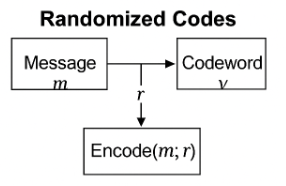
\includegraphics[width=0.4\linewidth]{Randomized.png}
    \caption{In randomized codes, the message is fixed first and fresh randomness is chosen each time to compute the codeword.}
    \label{fig:enter-label}
\end{figure}

\subsubsection{Self-Seeded Codes}
The randomness, $r$, is fixed before picking a message $m$ and thus, for arbitrary $m$, the code word $v$ is computed as before, $v \xleftarrow{}\textsf{Encode}(m; r)$. 

\begin{theorem}[Self-Seeded Codes]
    Assuming collision-resistant hash functions (CRHFs), $\exists$ efficiently computable self-seeded error detection and error correction codes for arbitrary polynomial-time adversarial errors with the following parameters: \begin{enumerate}
        \item Detection: For a constant $0 < \varepsilon < 1$, there is a code over a constant-sized alphabet with $R = 1 - \varepsilon$ that detects a $\rho = 1- \varepsilon$ fraction of errors
        \item Correction: For a constant $0 < \varepsilon < 1$ and $0 \leq \rho < 1/2 $, there is a code over a constant-sized alphabet with $R = 1 - \rho - \varepsilon$ that uniquely corrects $\rho$ fraction of errors
    \end{enumerate}
\end{theorem}

\begin{figure}[H]
    \centering
    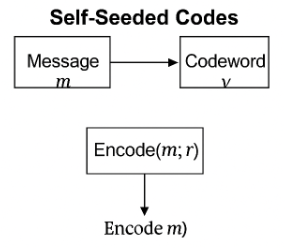
\includegraphics[width=0.4\linewidth]{SelfSeeded.png}
    \caption{In self-seeded codes, the randomness (seed) is fixed first, and the codeword is computed for each message using this fixed seed.}
    \label{fig:self-seeded-codes}
\end{figure}


\subsection{Construction}

The construction of both codes follow the same pattern and in fact, the only difference is that use of a hash function family $h_r$ needs to a one-way function for randomized codes and a collision-resistant hash function for self-seeded codes. As such, the construction that follows is generalized for both randomized and self-seeded codes. 

\subsubsection{Sub-Exponential Alphabet Detection}

Let $\mathcal{H} =\{h_r : \{0, 1\}^k \to \{0, 1\}^{\lambda}\}_{r \in \{0, 1\}^{\lambda}}$ be a family of hash functions with the desired properties. $\textsf{Encode}(m; r)$ creates a code $c$, defined as: $$c = ([m_1, r, h_r(m)], [m_2, r, h_r(m)], \ldots, [m_n, r, h_r(m)])$$ Where $m = (m_1, m_2, \ldots, m_n)$. This is interpreted at the receiver's end as: $$c' = ([m_1', r_1', y_1'], [m_2', r_2', y_2'], \ldots, [m_n', r_n', y_n'])$$ Given $c'$, $\mathsf{Decode}(c')$ does the following steps and checks: \begin{enumerate}
    \item Define $m' = (m_1', m_2', \ldots m_n')$
    \item Check if all $r_i'$ are the same
    \item Check if all $y_i'$ are the same and check if $y_i' = h_{r'_i}(m')$
\end{enumerate} If all checks pass, then output $m'$ otherwise output $\bot$. This scheme has a fairly large alphabet and the following scheme attempts to tackle that. 

\subsubsection{Constant Alphabet Detection}
\begin{wrapfigure}{r}{0.4\textwidth}
  \centering
  \vspace{-10pt}
  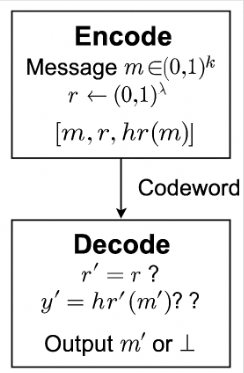
\includegraphics[width=0.4\textwidth]{LargeAlphabet.png}
  \caption{Constant Alphabet Detection Diagram}
  \vspace{-10pt}
\end{wrapfigure}
Let $(\textsf{Encode}_{ctrl}, \textsf{Decode}_{ctrl})$ be a standard error correcting code and the authors use this to define $c_{ctrl} = \textsf{Encode}_{ctrl}(r, h_r(m))$, effectively the second and third chunk from $(m_i, r, h_r(m))$ which was used in the previous construction but encoded. As such, $(m_i, r, h_r(m)) \mapsto (m_i, c_{ctrl})$ giving $c$ as: $$c = ([m_1, c_{ctrl}], [m_2, c_{ctrl}], \ldots, [m_n, c_{ctrl}])$$ This is interpreted at the receiver's end as: $$c' = ([m_1', c_{ctrl, 1}'], [m_2', c_{ctrl, 2}'], \ldots, [m_n,' c_{ctrl, n}'])$$ Given $c'$, $\textsf{Decode}(c')$ follows the exact same steps as before but first, it uses $\textsf{Decode}_{ctrl}$ to turn $c_{ctrl, i} \to (r_i', y_i')$. If any of the intermediary decodes, fail, then $\textsf{Decode}$ can output $\bot$. This relies on the correctness of the control code. \\\\\\\\\\\\



\subsubsection{Error Correction}
Let $(\textsf{Encode}_{data}, \textsf{Decode}_{data})$ be a list-decoding error correcting code and the authors use this to define $c_{data, i} = \textsf{Encode}_{data}(m_i)$ which replaces $m_i$ in the previous construction. As such, $c$ is now defined as: $$c = ([c_{data, 1}, c_{ctrl}], [c_{data, 2}, c_{ctrl}], \ldots, [c_{data, n}, c_{ctrl}])$$ This is interpreted as: $$c' = ([c_{data, 1}', c_{ctrl}'], [c_{data, 2}', c_{ctrl}'], \ldots, [c_{data, n}', c_{ctrl}'])$$ Given $c'$, $\textsf{Decode}(c')$ first recovers each $m_i$ using $\textsf{Decode}_{data}(c_{data}') = m;$. This isn't as trivial as simply unique decoding as it outputs a list of potential decodes but a simple check is to compute $m'$ and check if it matches $y'$ by checking against $h_{r'}(m') = y'$. This recovers $m$ and is based on the correctness of the underlying data code.  

\subsection{Correctness}

The general set of algorithms rely on the correctness of the underlying control and data error correcting codes however, under the specific code settings, that is, randomized and self-seeded, the correctness relies on specific properties of the hash family $\mathcal{H}$. In both cases, the primary idea is that regardless of message choice, it should be hard to come up with a message chunk $m_i'$ to replace $m_i$ such that $m' = (m_1, m_2, \ldots, m_i', \ldots, m_n)$ and $m = (m_1, m_2, \ldots, m_i, \ldots, m_n)$ where $m \neq m'$ but $h_r(m) = h_r(m')$. 

\begin{enumerate}
    \item Self-Seeded Codes require CRHFs: Since the randomness is fixed before the message is picked, the scheme requires $\mathcal{H}$ to be a collision resistant hash function as it ensures that for a given hash function $h_r$, finding two messages such that $m \neq m'$ but $h_r(m) = h_r(m')$ is hard for a polynomial time adversary
    \item Randomized Codes require Universal One Way Hash Functions (UOWHFs) which require OWFs: Since randomness is set after the message is picked, UOWHFs ensure that a polynomial time adversary cannot find $m'$ such that $m \neq m'$ but $h_r(m) = h_r(m')$
\end{enumerate}

\section{Exploring the 2025 Paper}

The biggest limitation of the 2024 work was that the constructions worked for sufficiently 
 large linear codes, that is $q \gg 2$ but the gold standard, if such a thing exists for EDAC schemes, is binary error detection and correction. In essence, larger alphabets by the very nature of including a lot symbols include a lot of information with every symbol which are, ultimately, encoded as bit strings. As such, the 2025 work by Jad Silbak and Daniel Wichs attempts to address this limitation, specifically for seeded codes. It should be noted that seeded codes are distinct from self-seeded / randomized codes explored in the previous work in that the seed in seeded codes is shared between both the encoding and decoding algorithm whereas in self-seeded / randomized codes, the seed is only used by the encoding algorithm. 

 \subsection{Selective Security vs. Adaptive Security}

 The goal of the adversary is to come up with codeword $v'$ such that $\Delta(v, v') \leq p$ for $v = \mathsf{Encode}_s(m)$ for some message $m$ and seed $s$ such that $v'$ does not decode to $m$. This, however, can be split into different cases depending on the order depending on when the adversary sees $s$, before or after picking $m$. 

 \subsubsection{Selective Security}

  Under the notion of selective security, the adversary picks $m$ before seeing $s$ and is given $\mathsf{Encode}_s(m) = v$. The adversary then picks $v'$ such that $\Delta(v, v') \leq p$ and the goal for the EDAC scheme remains as it was before: \begin{enumerate}
      \item Detection: if $v' = v$, $v'$ decodes to $m$ otherwise, if $v' \neq v$, $v'$ decodes to $\bot$ with overwhelming probability
      \item Correction: $v'$ decodes to $m$ with overwhelming probability 
  \end{enumerate} The construction presented in the paper creates a selectively secure seeded code using Learning with Errors (LWE). 

 \subsubsection{Adaptive Security}

  Under the notion of selective security, the adversary picks $m$ after seeing $s$. The adversary is then given $\mathsf{Encode}_s(m) = v$. The adversary then picks $v'$ such that $\Delta(v, v') \leq p$ and the goal for the EDAC scheme remains as it was before: \begin{enumerate}
      \item Detection: if $v' = v$, $v'$ decodes to $m$ otherwise, if $v' \neq v$, $v'$ decodes to $\bot$ with overwhelming probability
      \item Correction: $v'$ decodes to $m$ with overwhelming probability 
  \end{enumerate} The construction presented in the paper creates an adaptively secure seeded code using Dark Matter hash assumption. 

\subsection{Construction}
For all the constructions that follow, scheme's algorithms are denoted by $(\textsf{Encode}_s, \textsf{Decode}_s)$. 

\subsubsection{Selectively Secure Error Detection (SSED)}

Let $\mathcal{H} = \{h:\{0, 1\}^k \to \{0, 1\}^v\}$ be a family of T2CI hash functions. Let $\textbf{G} \in \mathbb{F}_2^{v \times n}$ be a generator matrix for linear efficiently list-decodable codes such that maps messages to codewords as $\textbf{G}: \{0, 1\}^v \to \{0, 1\}^n$ where $n = k +v$. Take $\textbf{G}$ and turn it into the full rank matrix $\textbf{A} \in \mathbb{F_2^{n \times n}}$ by completing the basis, thus $\textbf{A} = [\textbf{G} \text{ } \textbf{B}]^T$. The encoding algorithm, $\textsf{Encode}_s(m)$ is as follows: $$c = (m, h_s(m))\textbf{A} = m\textbf{B} + h_s(m)\textbf{G}$$ The decoding algorithm, $\textsf{Decode}_s(c')$, interprets $c$ as $c'$ which does the following steps: \begin{enumerate}
    \item Compute $(m' , y') = c' \textbf{A}^{-1}$
    \item Check $h_s(m') = y'$ and if true, output $m'$ as $m$ otherwise, output $\bot$ 
\end{enumerate}

\subsubsection{Selectively Secure Error Correction (SSEC)}

\begin{wrapfigure}{r}{0.48\textwidth}
  \centering
  \vspace{-10pt}
  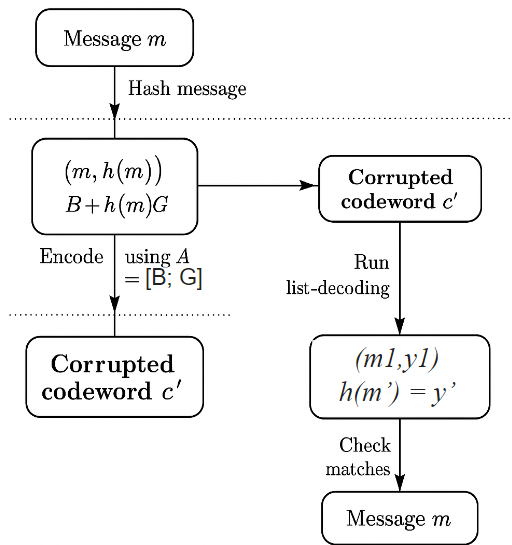
\includegraphics[width=0.46\textwidth]{Selective.png}
  \caption{Selectively Secure Error Correction (SSEC)}
  \vspace{-10pt}
\end{wrapfigure}

The construction is almost the same, however, instead of $n = v +k$ in $\textbf{G} \in \mathbb{F}_2^{v \times n}$, we have $n > v + k$ which means $\textbf{A} \in \mathbb{F}_2^{(v + k) \times n}$ given $\textbf{A}$ is defined as before, that is, $\textbf{A} = [\textbf{G} \text{ } \textbf{B}]^T$. Similarly, $\textsf{Encode}_s(m)$ remains the same so $c = m\textbf{B} + h_s(m)\textbf{G}$. The decoding algorithm $\textsf{Decode}_s(c')$ follows the following steps: \begin{enumerate}
    \item Applies list decoding over $c'$ to obtain a list of $(m', y')$ pairs 
    \item $\forall$ $(m', y')$ pairs, check if $h_s(m') = y'$, if yes, then $m'$ is the correct decoding otherwise output $\bot$\\\\\\\\\\\\\\\\
\end{enumerate}

\subsubsection{Adaptively Secure Error Detection (ASED)}


The authors construct an adaptively secure error detection seeded code under the Dark Matter hash assumption. The encoding algorithm $\textsf{Encode}_s(m)$ proceeds as follows:

\begin{enumerate}
    \item Map $m$ to $\tilde{m}$ via $\textsf{map}_{2 \to 3}: m \mapsto \tilde{m} \in \mathbb{F}_3^{\tilde{k}}$, where $\tilde{k} = \lceil (\log_3 2) \cdot k \rceil$.
    \item Sample $\mathbf{B} \leftarrow \mathbb{F}_3^{\tilde{k} \times l}$ with $l = (1 + \delta) \cdot \tilde{k}$ for some small $\delta > 0$, and compute $y = \tilde{m} \cdot \mathbf{B}$.
    \item Map $y$ to $\tilde{y}$ via $\textsf{map}_{3 \to 2}: y \mapsto \tilde{y} \in \mathbb{F}_2^{\tilde{l}}$, where $\tilde{l} = \lceil (\log_2 3) \cdot l \rceil$.
    \item Sample $\mathbf{A} \leftarrow \mathbb{F}_2^{\tilde{l} \times n}$ with $n = (1 + \delta) \cdot \tilde{l}$ and compute the final codeword $c = \tilde{y} \cdot \mathbf{A}$.
\end{enumerate}

In compact form, we have $\textsf{Encode}_s(m) = \textsf{map}_{3 \to 2}(\textsf{map}_{2 \to 3}(m) \cdot \mathbf{B}) \cdot \mathbf{A}$. The authors consider both $\mathbf{A}$ and $\mathbf{B}$ as part of the seed. The decoding algorithm $\textsf{Decode}_s(c')$ computes $m' = \textsf{Encode}_s^{-1}(c')$; if both matrices are invertible (which occurs with high probability), then $m' = m$, otherwise the decoder returns $\bot$.\\

\begin{figure}[H]
  \centering
  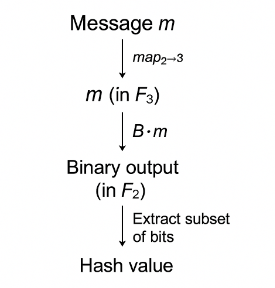
\includegraphics[width=0.4\textwidth]{AdaptiveHash.png}
  \caption{Adaptively Secure Error Detection (ASED)}
  \label{fig:ASED}
\end{figure}

\subsubsection{Adaptively Secure Error Correction (ASEC)}

Let $(\textsf{Encode}_{\mathsf{List}}, \textsf{Decode}_{\mathsf{List}})$ be an efficient list-encoding error-correcting code, and let \\ $(\textsf{Encode}'_s, \textsf{Decode}'_s)$ be an adaptively secure error detection code. Then the encoding algorithm is defined as $\textsf{Encode}_s(m) = \textsf{Encode}_{\mathsf{List}}(\textsf{Encode}'_s(m))$.

Since list decoding is used, $\textsf{Decode}_s(c')$ computes a list of candidate vectors $v$. If there exists a $v$ such that $\textsf{Decode}'_s(v) = m' \neq \bot$, then $m'$ is the correct message. If no valid decoding is found, the algorithm outputs $\bot$.\\



\subsection{Correctness}

\begin{enumerate}
    \item \textbf{SSED and SSEC.} When there are no errors in the received codeword, decoding succeeds via simple matrix inversion. If the received codeword has errors but the decoder does not output $\bot$, then it must be the case that $h_s(m) = h_s(m')$ for some $m \neq m'$, which implies:
    \[
    h(m')\mathbf{G} = (m - m')\mathbf{B} + h(m)\mathbf{G} + e
    \]
    This further implies $h(m') \in f(m, m', h(m))$, violating the T2CI assumption. Thus, if an adversary can find $m' \neq m$ that passes verification despite errors, the T2CI hash family is insecure. This argument extends to SSEC as well, in the context of error correction rather than detection.

    \item \textbf{ASED and ASEC.} Since both constructions rely on the Dark Matter hash assumption, they can be analyzed together. ASEC additionally uses a list-decoding scheme, which is assumed to be correct. The authors conjecture that the probability of finding a collision with $h_s$ is less than $\frac{2^{o(t)}}{2^t}$. If this conjecture holds, both error detection and correction follow by analogous reasoning to the SSED and SSEC cases.
    
\end{enumerate}

\section{Conclusion}

In this survey, we study two papers by Jad Silbak and Daniel Wichs that explore error detection and correction schemes under the notion of a computationally bounded adversarial communication channel. In the 2024 paper, the authors present constructions that use minimal assumptions, namely one-way functions and collision resistant hash functions in order to construct codes with large alphabets. The constructions include randomized and self-seeded codes where a seed $s$ is used only by the encoding algorithm. While the constructions are interesting, the use of large alphabets is not ideal as the gold standard for EDAC schemes is to come up with binary codes, that is, codes with alphabets made up of two symbols. In their 2025, this primary limitation is addressed. Under two notions of security, adaptive and selective, they construct seeded codes, that is, codes where both the encoding and decoding algorithms share a seed $s$ that use a binary alphabet using slightly more complicated assumptions, namely, the dark matter hash assumption. 

\section{Acknowledgments}

This project report / survey was prepared as part of the final project for Prof. Rishab Goyal’s COMP SCI 880: Topics in Theoretical Computer Science during the Spring 2025 semester. We are grateful to Prof. Goyal for his guidance, supervision, and for an engaging semester of cryptography. We would also like to thank Jad Silbak and Daniel Wichs for their interesting papers, which this survey seeked to study.
    
\newpage


\end{document}